\newgeometry{top=1cm, bottom=2cm, left=2cm, right=2cm}
\chapter{Initial System Design}
\label{ch:system_design}

\begin{figure}[H]
    \centering
    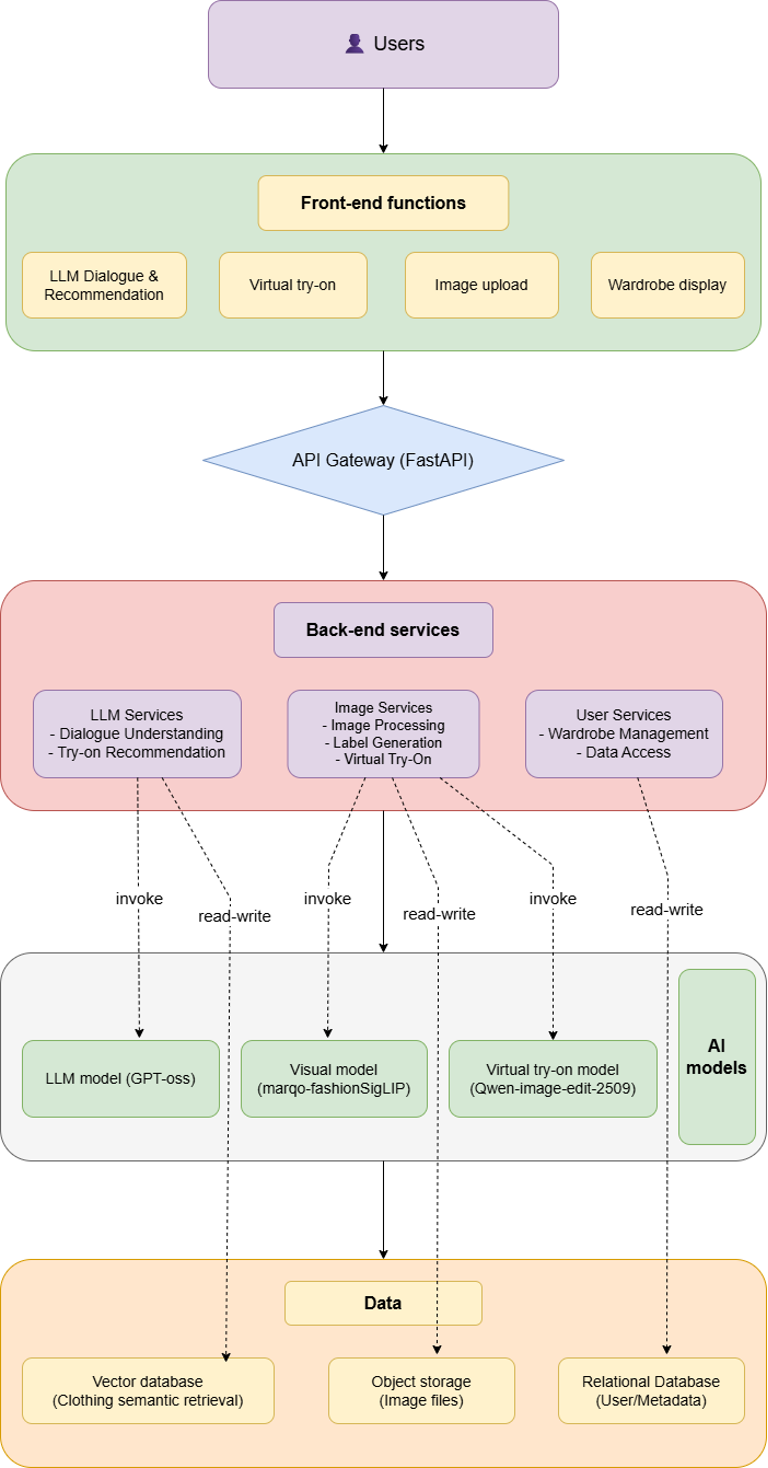
\includegraphics[width=0.6\textwidth]{images/Section_5/Full_Arch.png}
    \caption{System Architecture Diagram}
    \label{fig:system_architecture}
\end{figure}
\restoregeometry

\section{Module Decomposition}

\subsection{Front-end Module}
\begin{figure}[h]
    \centering
    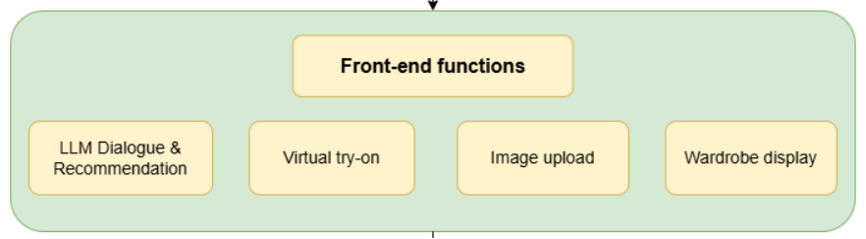
\includegraphics[width=0.8\textwidth]{images/Section_5/Front_end.png}
    \caption{Front-end Module}
    \label{fig:frontend_module}
\end{figure}
\textbf{Responsibility}\\[0.2cm]
The front-end provides interaction interfaces to end users, \textbf{enabling LLM dialog \& recommendations, image upload, virtual test, and wardrobe display}. It does not perform computational logic. Instead, it formats user actions into structured requests that are passed to the API Gateway.

\vspace{0.5cm}
\textbf{Input/Output}\\[0.3cm]
\textbf{Input:} user text queries, wardrobe actions, uploaded images, try-on selections\\[0.2cm]
\textbf{Output:} structured API requests, displayed results (images, recommendations, insights)

\vspace{0.5cm}
\textbf{Internal Components:}
\vspace{-0.3cm}
\begin{enumerate}
    \item \textbf{LLM Dialogue UI} - accepts natural language queries or refinement instructions from users
    \item \textbf{Wardrobe Display UI} - lists clothing items, metadata, and tags
    \item \textbf{Image Upload UI} - captures or uploads clothing/user images
    \item \textbf{Virtual Try-on UI} - renders generated preview and supports re-tries or saving
\end{enumerate}


\subsection{Back-end Module (Core Services)}

\begin{figure}[H]
    \centering
    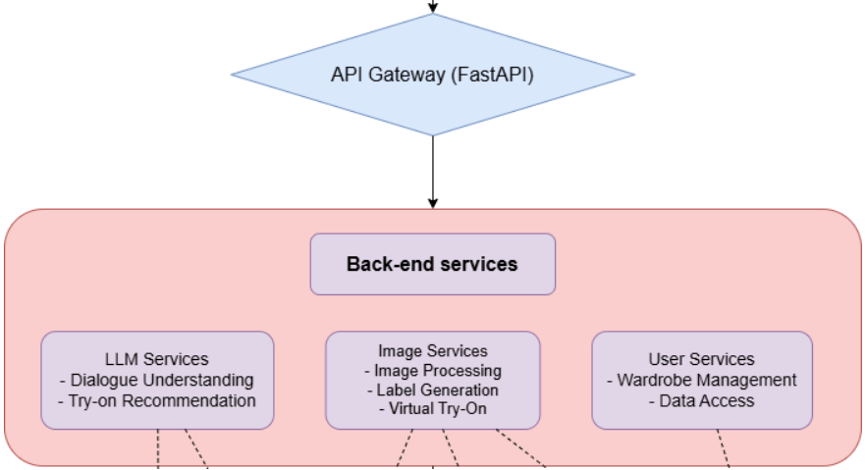
\includegraphics[width=0.8\textwidth]{images/Section_5/Back_end.png}
    \caption{Back-end Module (Core Services)}
    \label{fig:backend_module}
\end{figure}

The back-end implements business logic and orchestrates data flow. It exposes REST endpoints via \textbf{FastAPI}, serving as the single point of interaction between the front-end and the AI model layer.

\vspace{0.5cm}
\textbf{(1) LLM Services}
\textbf{Responsibility}
\vspace{-0.3cm}
\begin{enumerate}
    \item Parse user dialogue intent and extract recommendation parameters
    \item Generate outfit suggestions in natural language
    \item Provide structured semantic output (e.g., tags, colors, style descriptions)
    \item Integrate contextual factors such as weather or user preference history
\end{enumerate}

\textbf{Input/Output}\\[0.3cm]
\textbf{IN:} user text, behavior history, wardrobe metadata\\[0.2cm]
\textbf{OUT:} outfit descriptions, item candidates, reasoning text, retrieval tags

\newpage

\textbf{(2) Image Services}
\textbf{Responsibility}
\vspace{-0.3cm}
\begin{enumerate}
    \item Extract semantic representations of clothing images and generate attribute labels (e.g., color, category, aesthetics)
    \item Prepare assets for virtual try-on
    \item Perform normalization and preprocessing on raw images
\end{enumerate}

\textbf{Interaction Flow}\\
Receives images $\rightarrow$ invoke model $\rightarrow$ stores extracted embeddings/labels

\vspace{0.5cm}


\textbf{(3) User Services}
\textbf{Responsibility}
\vspace{-0.3cm}
\begin{enumerate}
    \item Manage wardrobe structure
    \item Handle CRUD operations on items
    \item Retrieve filtered clothing items for downstream tasks
    \item Provide metadata for analytics and profile generation
\end{enumerate}

This service layer guarantees that the model modules never directly read or write data.

\newpage
\subsection{AI Model Layer}
\begin{figure}[h]
    \centering
    
\includegraphics[width=0.8\textwidth]{images/Section_5/AI_models.png}
    \caption{AI Model Layer}
    \label{fig:ai_model_layer}
\end{figure}

This layer performs heavy computation and is stateless from the system's perspective. Back-end services invoke model APIs; the system never embeds model logic in UI or database components.

\textbf{(1) GPT-oss}
\begin{enumerate}
    \item Dialogue understanding
    \item Recommendation generation
    \item Tag suggestion and structured output
\end{enumerate}

Carefully edited prompts allow the LLM to generate structured output, ensure that recommended tags conform to the system's predefined taxonomy. In the future, we can implement a Retrieval-Augmented Generation (RAG) framework to make the LLM's responses more accurate, reliable, and controllable.

\textbf{(2) Marqo-fashionSigLIP (Visual Embedding Model)}
\begin{enumerate}
    \item Per-item representation learning
    \item Semantic label extraction
    \item Category and pairing inference
\end{enumerate}

The model generates labels which are indexed into a database, enabling fast retrieval of compatible clothing items for LLM or recommendation logic.

\textbf{(3) Qwen-image-edit-2509 (Virtual Try-on Model)}
\begin{enumerate}
    \item Person--clothing compositing
    \item Outfit replacement on user photos or mannequin templates
\end{enumerate}

The model interprets predefined prompts into consistent image outputs, ensuring visual realism and minimizing artifacts.

\subsection{Data Layer}
\begin{figure}[H]
    \centering
    
\includegraphics[width=0.8\textwidth]{images/Section_5/Data.png}
    \caption{Data Layer}
    \label{fig:data_layer}
\end{figure}

\textbf{\large Object Storage}\\[0.2cm]
Object storage is used to store raw image assets, including original wardrobe uploads, virtual try-on preview images, and historical generated outputs. The back-end maintains only URIs or corresponding metadata rather than storing image directly. This approach improves scalability and ensures storage independence from application logic.\\

\textbf{\large Relational Database}\\[0.2cm] 
The relational database stores structured entities such as user accounts, clothing metadata, tags and attributes, and usage statistics. A relational schema provides predictable retrieval and analytical querying capabilities, while preventing excessive load on the embedding layer and avoiding semantic ambiguity.\\

\textbf{\large Vector Database}\\[0.2cm]
The vector database holds embedding representations of clothing items and supports fashion similarity search, style-based retrieval, and recommendation refinement. By enabling contextual semantic queries, such as "find neutral tops compatible with black trousers"—the system can deliver personalized and style-aware recommendations that extend beyond simple keyword matching.


\subsection{Module Interaction Summary}
\label{chapter: Module Interaction Summary}
The modules follow a clean isolation pattern:
\begin{enumerate}
    \item Front-end $\rightarrow$ API Gateway $\rightarrow$ Back-end
    \item Back-end $\rightarrow$ AI Models (invoke) $\rightarrow$ Data Layer (read/write)
    \item Models never access data directly
    \item Front-end never calls models directly
\end{enumerate}

\newpage




\section{Key User–Service Interactions (Sequence Diagrams)}
\textbf{\large 1. Virtual Try-on Sequence\\ (corresponding to UC-05 Virtual Try-on)}
\begin{figure}[H]
    \centering
    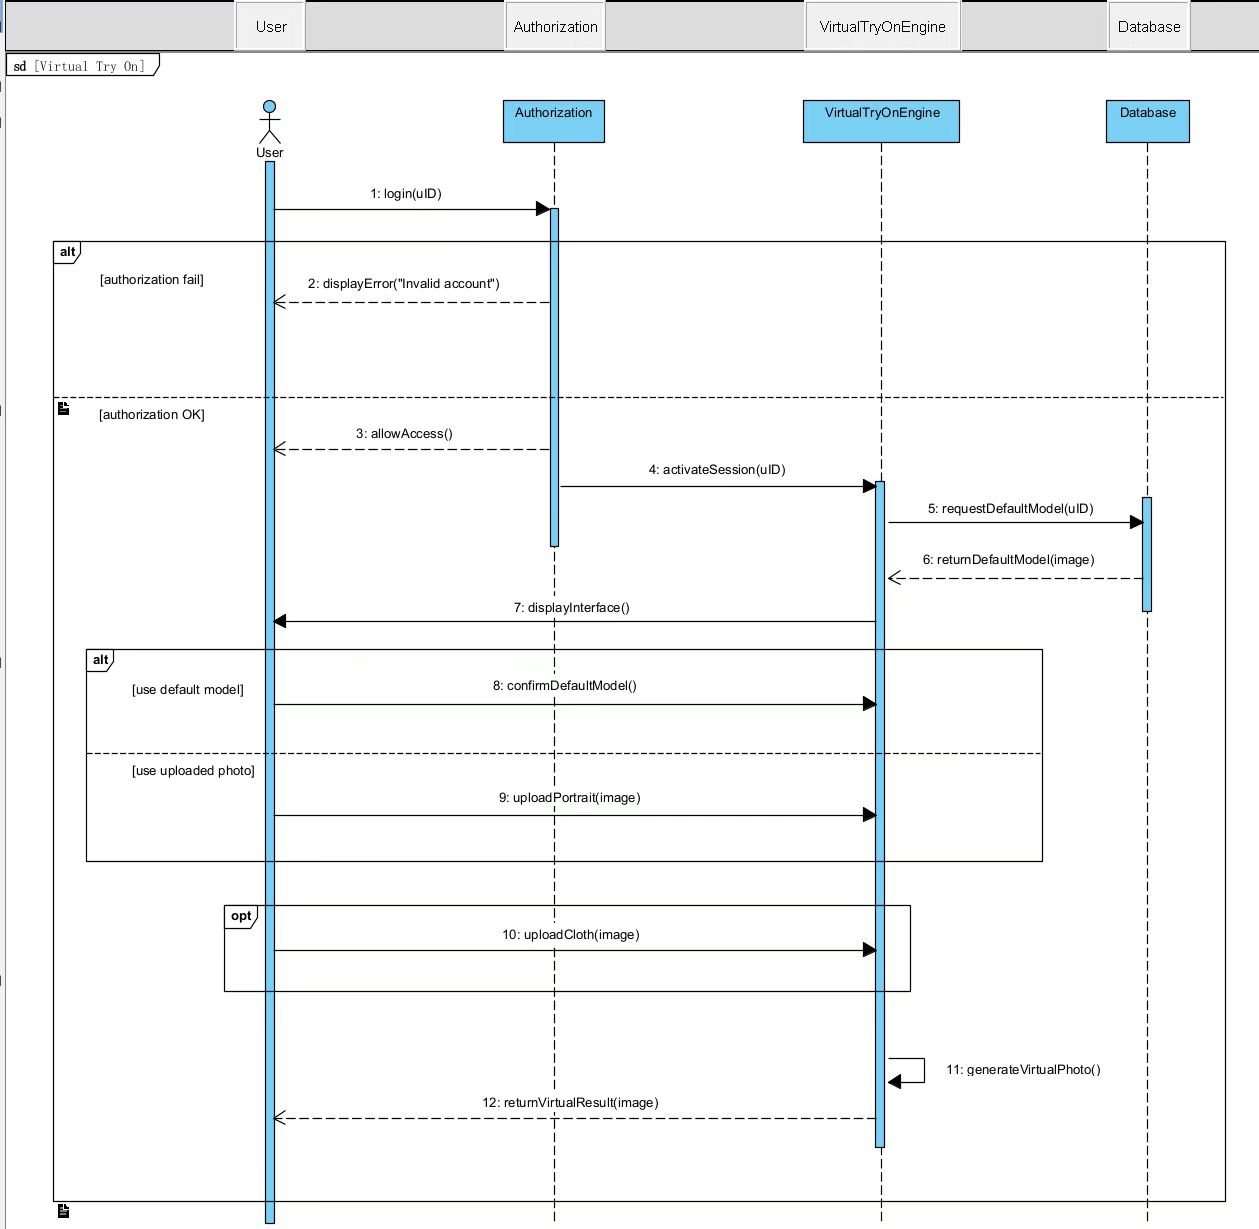
\includegraphics[width=1\textwidth]{images/Section_5/Sequence/Try_on.jpg}
    \caption{Virtual Try-on sequence diagram}
    \label{fig:Virtual try-on}
\end{figure}

\textbf{Justification \& link to requirements}\\
This sequence diagram illustrates that the try-on engine is encapsulated in the backend service, and the front end only sends images and parameters without directly interacting with the model, which achieves the constraint mentioned in \ref{chapter: Module Interaction Summary}.

It supports the virtual try-on of user photos (FR-10) and the virtual try-on of clothing images (FR-11), and connects with the subsequent process of exporting and sharing the try-on results (FR-12).\\


\textbf{\large 2. LLM Recommendation Sequence\\ (corresponding to UC-03 Get Outfit Recommendation \& UC-04 Provide Feedback) }
\begin{figure}[H]
    \centering
    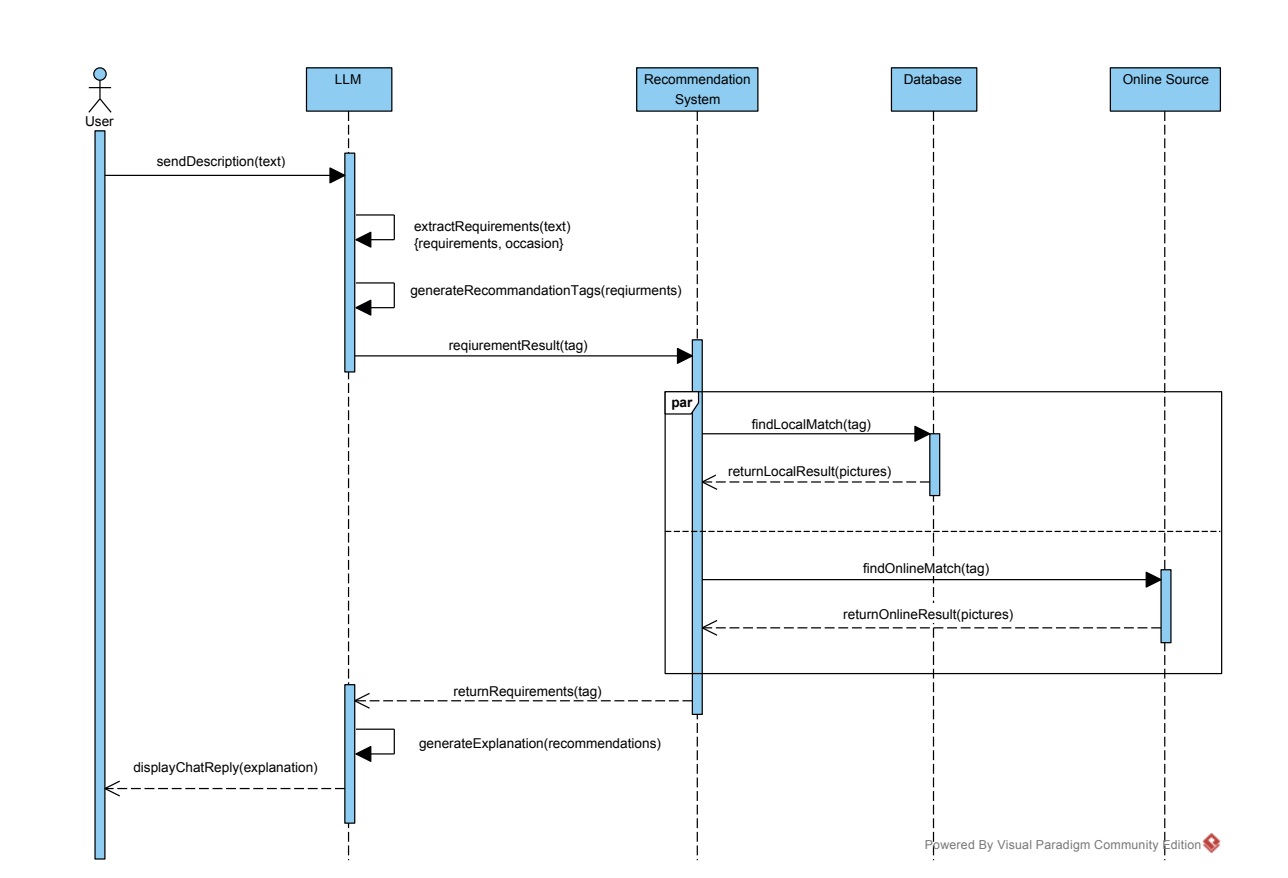
\includegraphics[width=1\textwidth]{images/Section_5/Sequence/Recommend.png}
    \caption{LLM Recommendation sequence diagram}
    \label{fig:Recommend}
\end{figure}

\textbf{Justification \& link to requirements}\\
This sequence diagram demonstrates the consistency between the recommendation process and the high-level architecture: front-end conversation → LLM service → recommendation system → data layer/external resources, and then back to the user interface, without any layer-over-layer access. 

It implements FR-04 user preference profiling, FR-05 input of occasion and constraints, FR-06 weather data acquisition, FR-07 outfit recommendation, and FR-08 recommendation explanation and alternative options; combined with the subsequent user feedback process, it also provides interfaces for FR-09 feedback loop and learning.\\


\newpage
\textbf{\large 3. Wardrobe Management Sequence\\ (Corresponding to UC-02 Manage Digital Wardrobe) }
\begin{figure}[H]
    \centering
    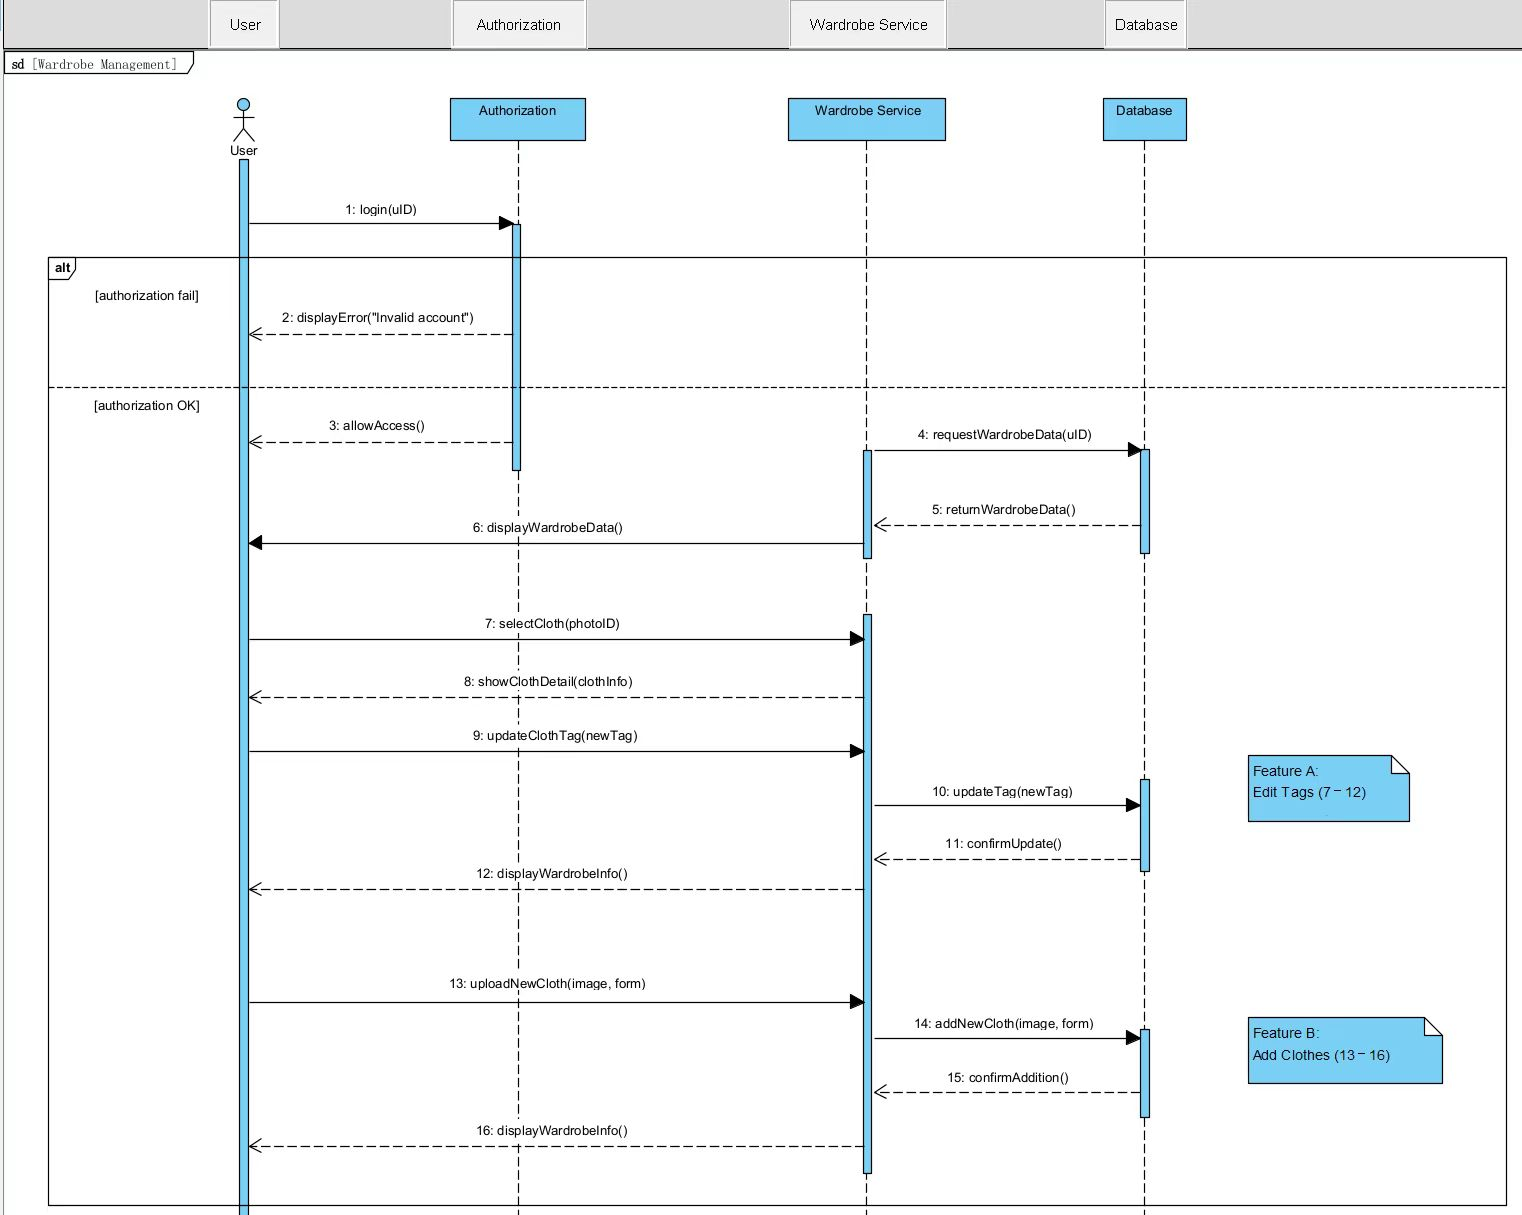
\includegraphics[width=1\textwidth]{images/Section_5/Sequence/Wardrobe_manage.jpg}
    \caption{Wardrobe Management sequence diagram}
    \label{fig:Wardrobe_management}
\end{figure}

\textbf{Justification \& link to requirements}\\
This sequence diagram illustrates the design where the front end accesses the data layer only through the service layer, which conforms to the layered architecture described in \ref{chapter: Module Interaction Summary}. 

It directly implements FR-01 account login, FR-02/FR-03 wardrobe creation (forms and images), and FR-13 wardrobe maintenance (query, filtering, batch editing), proving that the core wardrobe management function is feasible at the system level.\\


\newpage
\textbf{\large 4. Wardrobe Analysis Sequence\\ (Corresponding to UC-07 View/Edit User Profile)}
\begin{figure}[H]
    \centering
    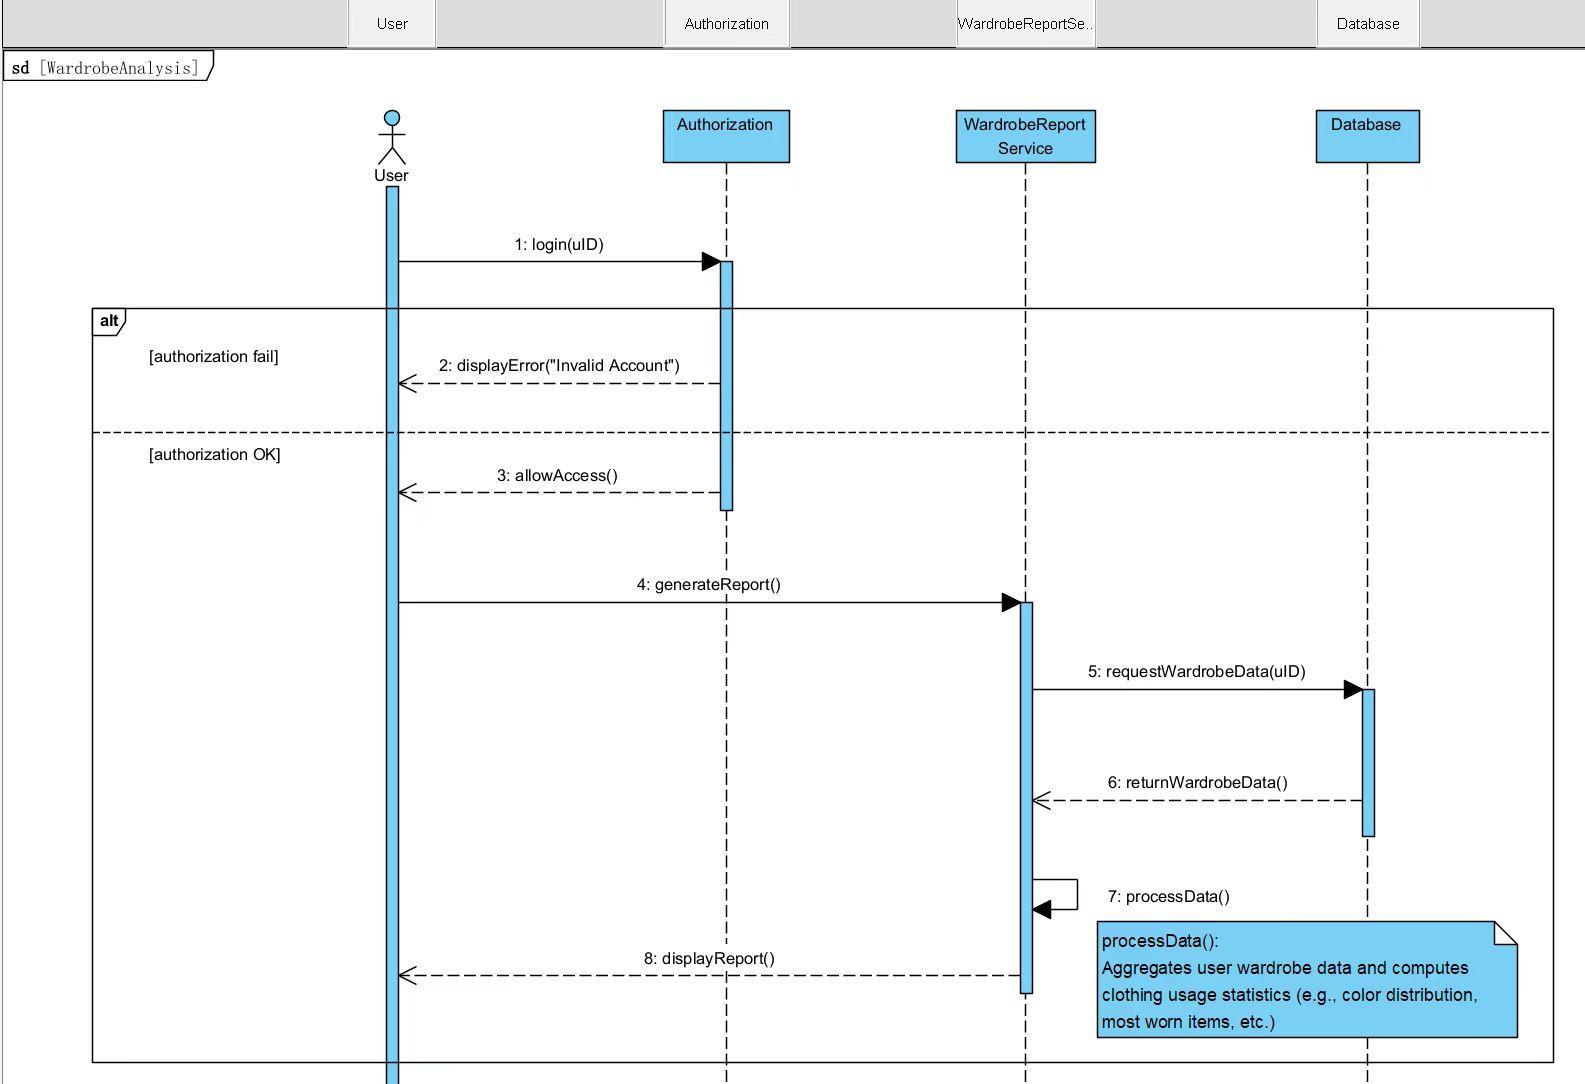
\includegraphics[width=1\textwidth]{images/Section_5/Sequence/Wardrobe_analysis.jpg}
    \caption{Wardrobe Analysis sequence diagram}
    \label{fig:Wardrobe_analysis}
\end{figure}

\textbf{Justification \& link to requirements}\\
This sequence diagram illustrates that preference profile is accomplished through independent analysis services, decoupled from ordinary CRUD operations. 

It realizes and supports the requirements for historical records and statistical views in FR-04 User Preferences (Profile Generation and Display) and FR-13 Wardrobe Maintenance, providing a data foundation for subsequent recommendations and visual analysis.\\

\newpage

\section{Database Schema and Storage Structure}
We propose a relational database schema (PostgreSQL) as an initial design to support structured user wardrobe data. The following tables illustrate key entities and their relationships.

The schema may evolve as the implementation progresses.


\subsubsection{Users Table}
\begin{itemize}
    \item \texttt{user\_id} (Primary Key, UUID) - Universally Unique Identifier serving as the primary key for user identification
    \item \texttt{username} (VARCHAR) - User's display name for profile identification
    \item \texttt{password\_hash} (VARCHAR) - Securely encrypted password digest using bcrypt/Argon2 algorithm
    \item \texttt{email} (VARCHAR, Unique) - Unique email address for authentication and communication
    \item \texttt{preference\_tags} (JSON) - Structured JSON object storing user's fashion style preferences and taste profiles
    \item \texttt{role} (ENUM('user', 'admin')) - Access control level defining user permissions within the system
    \item \texttt{created\_at} (TIMESTAMP) - Audit timestamp recording when the user account was initially created
    \item \texttt{updated\_at} (TIMESTAMP) - Audit timestamp tracking the last modification to user profile data
\end{itemize}


\subsubsection{Wardrobe Items Table}
\begin{itemize}
    \item \texttt{item\_id} (Primary Key, UUID) - Unique identifier for each clothing item in the system
    \item \texttt{user\_id} (Foreign Key) - References the owner user, establishing the user-item relationship
    \item \texttt{category} (ENUM('top', 'bottom', 'shoes', 'accessories', 'outerwear')) - Broad classification of clothing type for basic filtering
    \item \texttt{subcategory} (VARCHAR) - Specific item type description (e.g., 't-shirt', 'jeans', 'dress')
    \item \texttt{color} (VARCHAR) - Main color information for color-based matching and filtering
    \item \texttt{brand} (VARCHAR) - Clothing brand name for brand recommendations
    \item \texttt{style\_tags} (JSON) - AI-generated semantic style attributes (e.g., ["bohemian", "minimalist", "vintage"])
    \item \texttt{image\_url} (VARCHAR) - File path reference to the item image in cloud object storage
    \item \texttt{embedding\_vector} (VECTOR) - Mathematical vector representation for visual similarity search and compatibility matching
    \item \texttt{created\_at} (TIMESTAMP) - Time stamp recording when the item was added to the wardrobe
\end{itemize}


\subsubsection{Outfits Table}
\begin{itemize}
    \item \texttt{outfit\_id} (Primary Key, UUID) - Unique identifier for each saved outfit combination
    \item \texttt{user\_id} (Foreign Key) - References the owner user, establishing the user-outfit relationship
    \item \texttt{outfit\_name} (VARCHAR) - User-defined descriptive name for the outfit (e.g., "Weekend Casual")
    \item \texttt{outfit\_description} (TEXT) - LLM-generated natural language description explaining the outfit's style and rationale
    \item \texttt{items} (JSON) - Array of elements \_ids representing the complete clothing combination in this outfit
    \item \texttt{occasion} (VARCHAR) - Contextual label defining suitable events (e.g., 'casual', 'formal', 'business')
    \item \texttt{weather\_context} (JSON) - Structured weather parameters (temperature, season, conditions) for contextual recommendations
    \item \texttt{aesthetic\_score} (FLOAT) - A numerical rating evaluating the visual appeal and coherence of the outfit
    \item \texttt{created\_at} (TIMESTAMP) - Timestamp recording when the outfit was created or saved
\end{itemize}

\subsubsection{TryOn Sessions Table}
\begin{itemize}
    \item \texttt{session\_id} (Primary Key, UUID) - Unique identifier for each virtual try-on session
    \item \texttt{user\_id} (Foreign Key) - References the user who performed the try-on operation
    \item \texttt{original\_image\_url} (VARCHAR) - File path to the user's base photo used as the try-on foundation
    \item \texttt{garment\_id} (Foreign Key) - References the specific clothing item from the wardrobe that was virtually tried on
    \item \texttt{tryon\_image\_url} (VARCHAR) - File path to the AI-generated image showing the virtual try-on result
    \item \texttt{prompt\_used} (TEXT) - Custom text prompt provided by the user or system to guide the try-on generation process
    \item \texttt{created\_at} (TIMESTAMP) - Timestamp recording when the virtual try-on session was executed
\end{itemize}

\subsubsection{Dialogue Sessions Table}
\begin{itemize}
    \item \texttt{session\_id} (Primary Key, UUID) - Unique identifier for each conversation session with the AI assistant
    \item \texttt{user\_id} (Foreign Key) - References the user who engaged in the dialogue session
    \item \texttt{query\_text} (TEXT) - Complete natural language input provided by the user seeking fashion advice or recommendations
    \item \texttt{llm\_response} (TEXT) - Full response generated by the GPT-oss model addressing the user's query
    \item \texttt{recommended\_items} (JSON) - Array of item IDs from the user's wardrobe that were recommended during the dialogue
    \item \texttt{timestamp} (TIMESTAMP) - Exact date and time when the dialogue interaction occurred
\end{itemize}



\section{Initial UI Design}
\label{chapter_ui_design}
\begin{figure}[H]
    \centering
    % 左图
    \begin{minipage}[b]{0.48\textwidth}
        \centering
        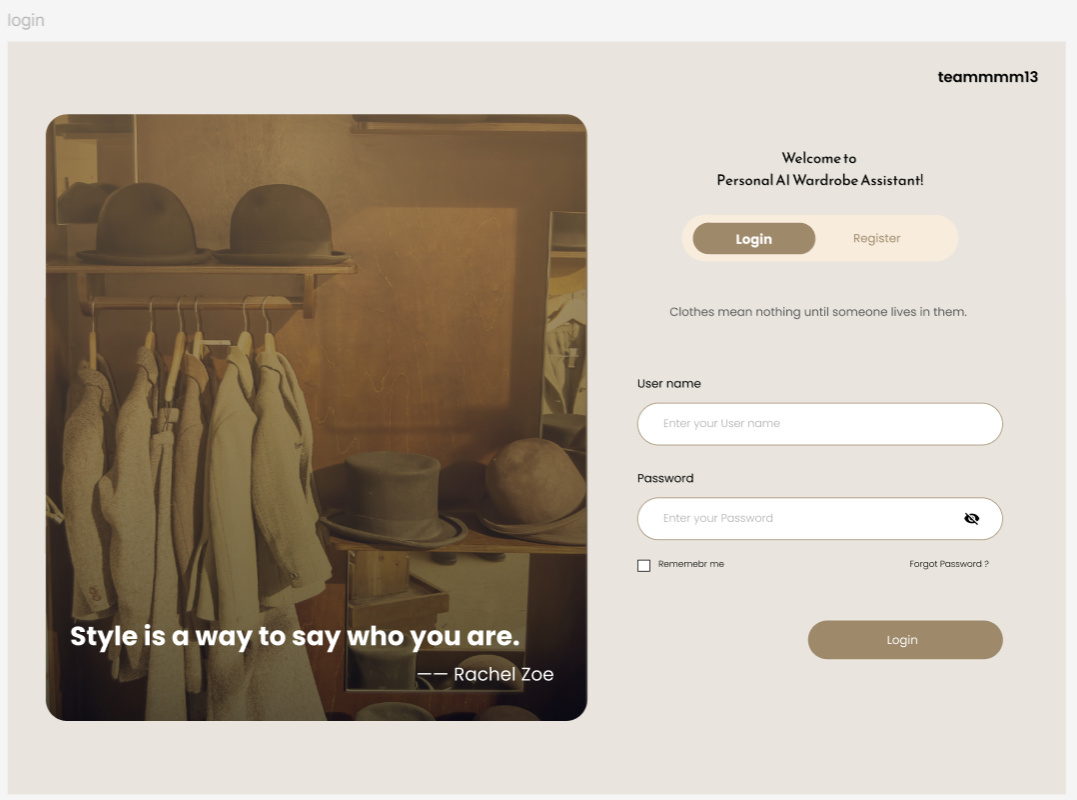
\includegraphics[width=\textwidth]{images/Section_5/UI/login.png}
        \caption*{Login UI}
    \end{minipage}
    \hfill
    % 右图
    \begin{minipage}[b]{0.48\textwidth}
        \centering
        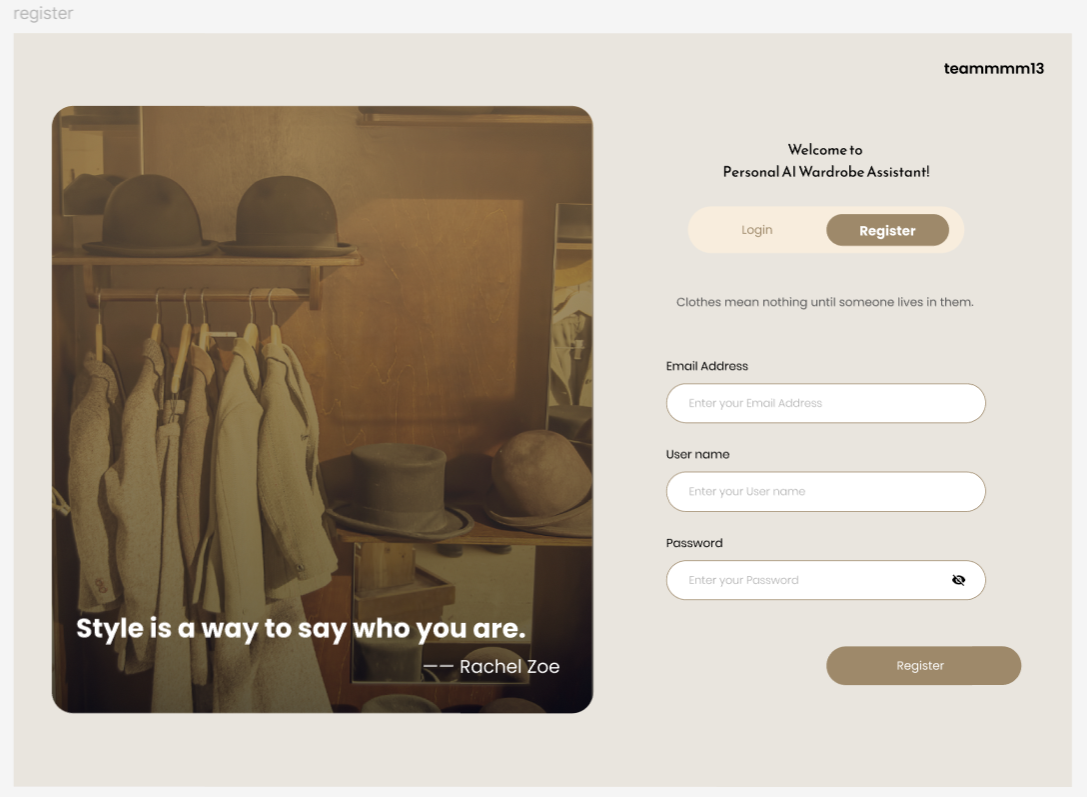
\includegraphics[width=\textwidth]{images/Section_5/UI/register.png}
        \caption*{Register UI}
    \end{minipage}
    \caption{login page (left) and register page (right)}
    \label{fig:ui_login_recommendation}
\end{figure}

\textbf{\large Visual theme}:\\[0.5cm]
The overall interface adopts a warm color combination of cream and warm brown. The background is a light grayish beige, while the main buttons and titles are highlighted in a darker warm brown and caramel color. 

We were inspired by the colors of traditional wooden closets, and aim to create a gentle and non-distracting visual atmosphere, while reducing the coldness of the software as a tool.\\


\textbf{\large Layout structure of main pages}:\\[0.5cm]
All pages adopt a two-column layout: the left column lists the main functions, while the right column presents the specific interfaces of each function, ss shown in Fig \ref{fig:initial_ui}.

\begin{figure}[H]
    \centering
    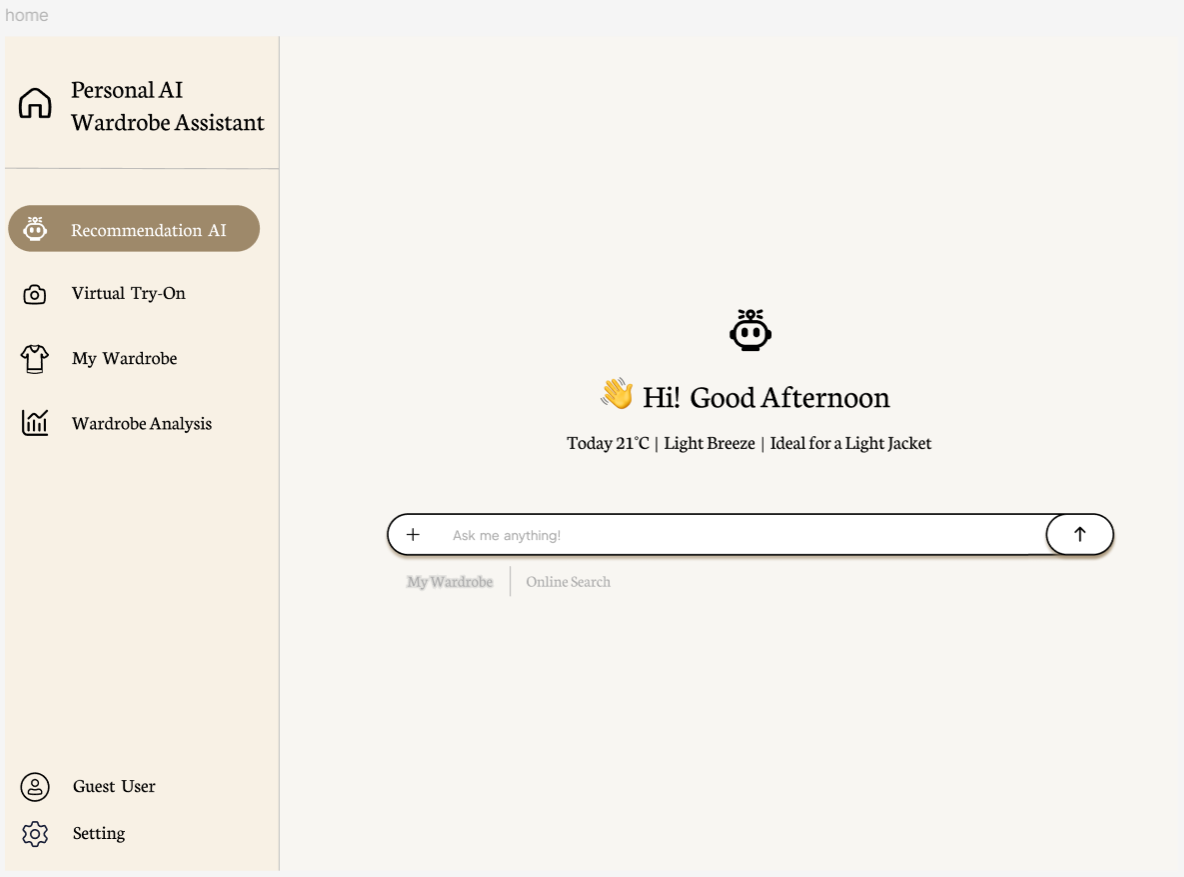
\includegraphics[width=0.6\textwidth]{images/Section_5/UI/initial.png}
    \caption{Initial page}
    \label{fig:initial_ui}
\end{figure}

Below is an introduction to the UI of the four pages of main functions of this software:
\begin{itemize}
\item \textbf{LLM Recommendation}
\begin{figure}[H]
    \centering
    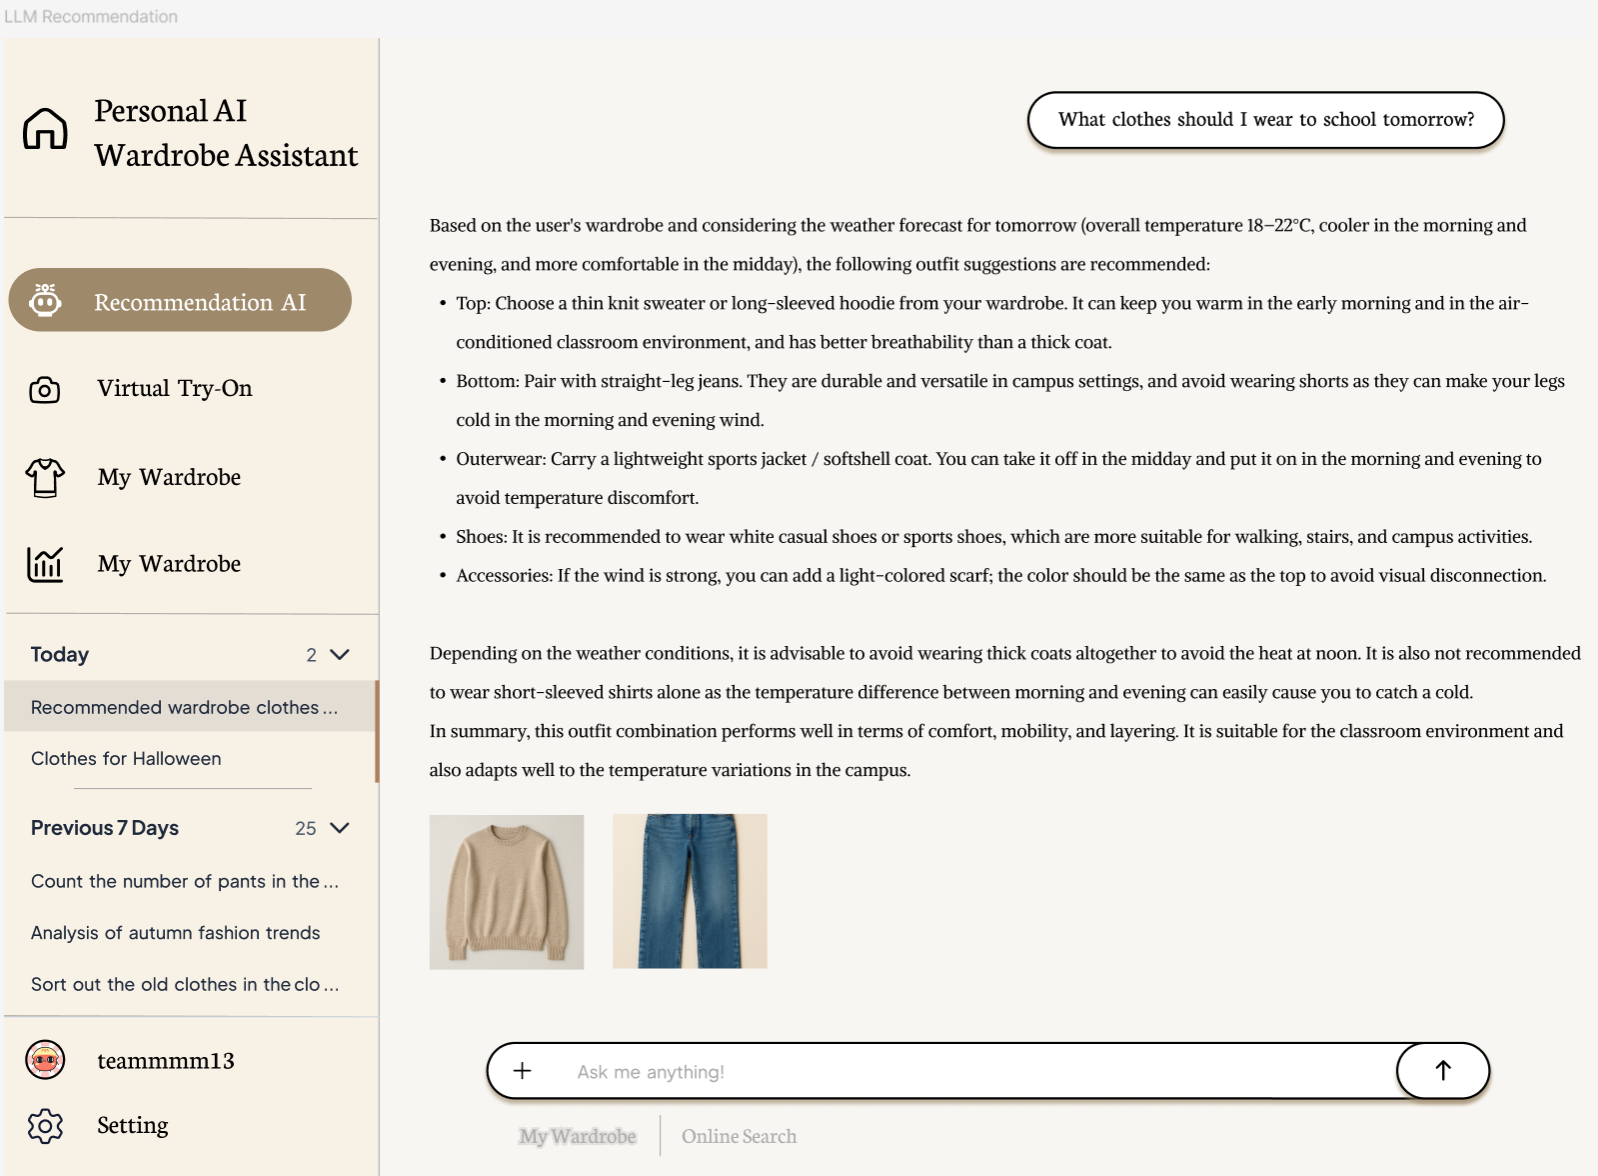
\includegraphics[width=0.6\textwidth]{images/Section_5/UI/LLM.png}
    \caption{LLM Recommendation page}
    \label{fig:llm_ui}
\end{figure}
The left sidebar of the LLM page builds on the existing navigation and also presents the user’s query history in chronological order.
The right column displays the detailed recommendations generated by the language model.\\

\item \textbf{Virtual Try-On}
\begin{figure}[H]
    \centering
    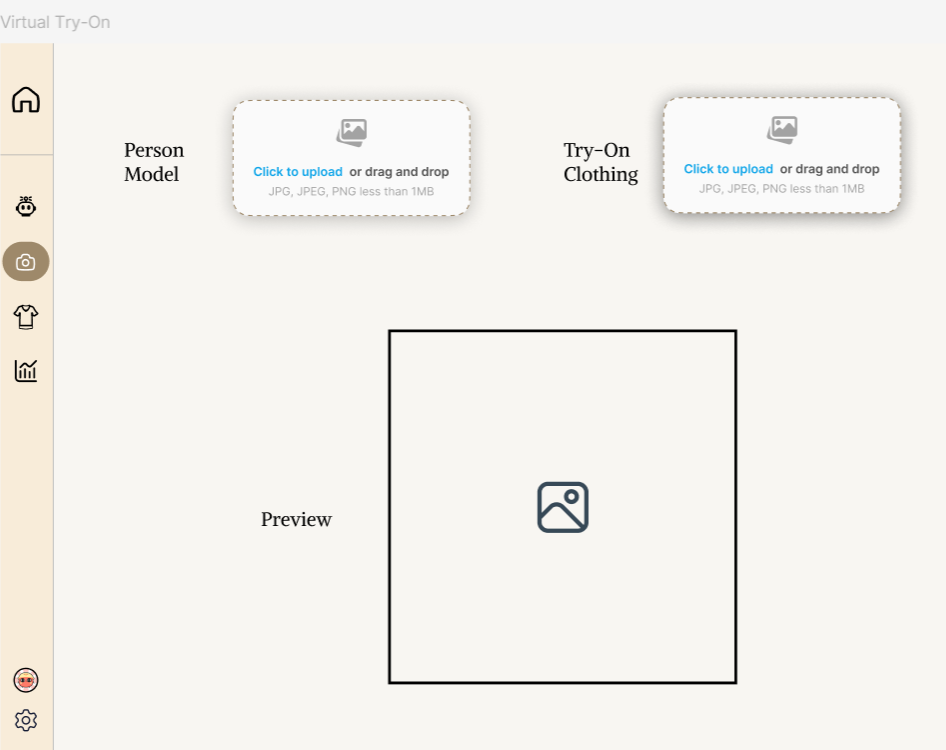
\includegraphics[width=0.6\textwidth]{images/Section_5/UI/VTO.png}
    \caption{Virtual Try-On page}
    \label{fig:VTO_ui}
\end{figure}
The main page features two upload cards at the top—one for the user's body model and another for clothing images. A large central preview panel below shows the try-on result.

The entire layout prioritizes clarity and usability, providing users with a simple workflow guide: upload → generate → preview.\\

\item \textbf{Wardrobe Management}
\begin{figure}[H]
    \centering
    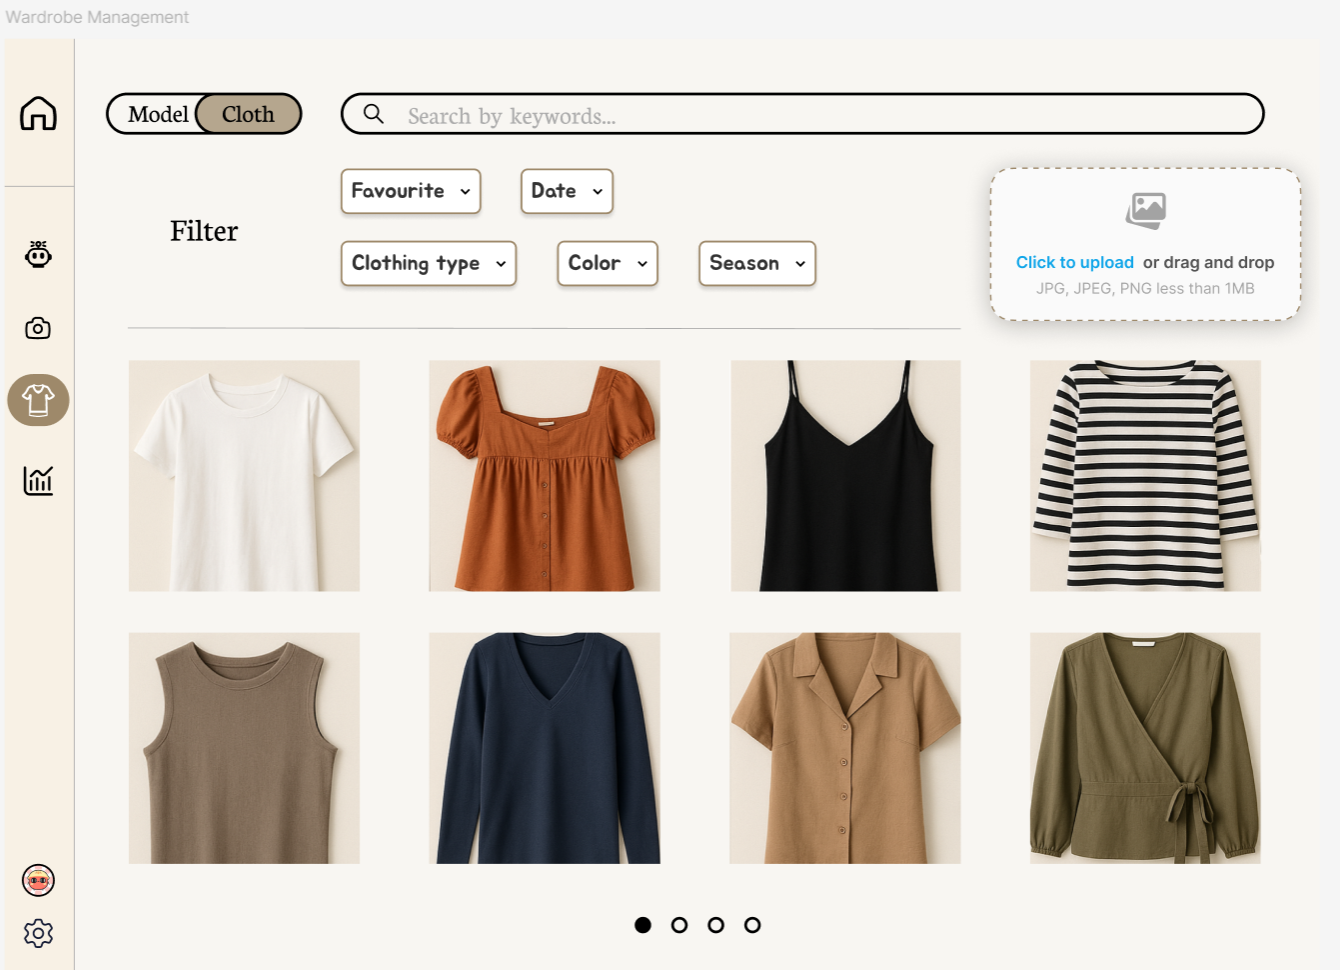
\includegraphics[width=0.6\textwidth]{images/Section_5/UI/management.png}
    \caption{Wardrobe Management page}
    \label{fig:management_ui}
\end{figure}
The top of the Wardrobe Management page includes a Model/Cloth toggle button, a search bar, and an upload card. Below, users can refine the search results through multiple dropdown menus. Clothing items are displayed in a uniform grid, with pagination at the bottom for browsing more entries.\\

\item \textbf{Wardrobe Analysis}
\begin{figure}[H]
    \centering
    
\includegraphics[width=0.6\textwidth]{images/Section_5/UI/analysis.png}
    \caption{Wardrobe Analysis page}
    \label{fig:Wardrobe_analysis_ui}
\end{figure}
The Wardrobe Analysis page adopts an information-intensive dashboard layout. This area presents the wardrobe data indicators through multiple independent information cards. Each card focuses on a separate wardrobe KPI, enables users to quickly understand the wardrobe situation from a global perspective.

\end{itemize}
